\documentclass{beamer}
\usepackage{beamerthemeshadow}
\usepackage{verbatim}

\usepackage{lastpage}
\usepackage{xcolor}
\usepackage{pgf}
\usepackage{colortbl}

\newcommand{\bi}{\begin{itemize}}
\newcommand{\ei}{\end{itemize}}
\newcommand{\be}{\begin{enumerate}}
\newcommand{\ee}{\end{enumerate}}
\newcommand{\bd}{\begin{description}}
\newcommand{\ed}{\end{description}}
\newcommand{\prbf}[1]{\textbf{#1}}
\newcommand{\prit}[1]{\textit{#1}}
\newcommand{\beq}{\begin{equation}}
\newcommand{\eeq}{\end{equation}}
\newcommand{\bdm}{\begin{displaymath}}
\newcommand{\edm}{\end{displaymath}}

\newcommand{\ft}[1]{
  \frametitle{\begin{tabular}{p{4.2in}r} \textcolor{white}{#1} & \small{\insertframenumber / \inserttotalframenumber} \end{tabular}}
  \setbeamercovered{transparent=18}
}

\newcommand{\stepinv}{\setbeamercovered{invisible}}
\newcommand{\stopinv}{\setbeamercovered{transparent=18}}
\newcommand{\uncoverinv}[1]
{
  \setbeamercovered{invisible}
  \uncover<+->{#1}
  \setbeamercovered{transparent=18}
}
\newcommand{\ans}[1]{\textcolor{blue}{#1}}
\newcommand{\ansinv}[1]
{
  \setbeamercovered{invisible}
  \uncover<+->{\textcolor{blue}{#1}}
  \setbeamercovered{transparent=18}
}
\newcommand{\setinv}{\setbeamercovered{invisible}}
\newcommand{\setvis}{\setbeamercovered{transparent=18}}
\newcommand{\centerpic}[2]
{
  \begin{center}
  \includegraphics[#1]{#2}
  \end{center}
}
\newcommand{\h}[1]{\hat{#1}}
\newcommand{\ds}{\displaystyle}

\definecolor{light}{rgb}{1.0,0.5,0.5}
\newcommand{\hl}[1]{\alt<#1>{\rowcolor{light}\hspace*{-2.1pt}} {\hspace*{-2.1pt}} }

\definecolor{mycolor}{rgb}{0.56,0.28,0.56}
\usecolortheme[named=mycolor]{structure}

\title[Initial Expectations in New Keynesian Models with Learning]{Initial Expectations in New Keynesian Models with Learning}
\author[Winona State University. February 2009.]{James Murray\\Dahl School of Business\\Viterbo University}
\date{February 4, 2009}

\begin{document}

\frame{\titlepage}
\setcounter{framenumber}{0}

\section{}
\subsection{Purpose}
\frame
{
  \ft{Purpose}
  \bi
  \item<+-> Purpose: Determine how learning vs. rational expectations affects our empirical understanding of a standard monetary economics model.
  \item<+-> \textbf{Learning}: type of adaptive expectations.
  \item<+-> \textbf{Rational Expectations}: assumes perfect knowledge of how the economy works, expectations do not evolve.
  \item<+-> \textbf{New Keynesian Monetary Model}:
    \bi
    \item<+-> Most commonly used model in monetary economics literature.
    \item<+-> Provides an explanation for how real GDP, inflation, and the federal funds rate are related.
    \ei
  \ei
}

\section{Monetary Framework}
\subsection{Types of Expectations}
\frame
{
  \ft{Rational Expectations}
  \bi
  \item<+-> Most common assumption in macroeconomic theory and empirical evaluation of macroeconomic models.
  \item<+-> Agents know entire structure of the economy.
  \item<+-> Agents know all parameters that govern consumer and producer behavior:
    \bi
    \item<+-> Elasticity of labor supply, intertemporal elasticity of substitution, degree of price flexibility, behavior of monetary policy, etc.
    \ei
  \item<+-> Stochastic uncertainty: unexpected shocks can still hit the economy.
  \item<+-> Lots of authors have estimated RE monetary models: Ireland (2004, 2006), Rotemburg and Woodford (1997), Smets and Wouters (2003, 2005, 2007).
  \ei
}

\frame
{
  \ft{Least Squares Learning}
  \bi
  \item<+-> Agents do not know structure of the economy.
  \item<+-> Agents form expectations by running regressions.
  \item<+-> Example: Predicting future inflation
    \bi
    \item<+-> Explanatory variables: past inflation, past output, past interest rates.
    \item<+-> Regression equation:
    \uncover<+->{\bdm \hat{\pi}_{t+1} = \beta_{0} + \beta_{1} \pi_{t} + \beta_{2} y_{t} + \beta_{3} r_{t}\edm}
    \item<+-> $\hat{\pi}_{t+1}$: expectation of future inflation.
    \item<+-> $\pi_t$: inflation at time $t$
    \item<+-> $y_t$: output at time $t$
    \item<+-> $r_t$: federal funds rate at time $t$
    \ei
  \ei
}

\subsection{New Keynesian Model}
\frame
{
  \ft{New Keynesian Model: Optimal Consumer Behavior}
  \bi
  \item<+-> Consumers maximize net present value of lifetime utility, subject to their budget constraint.
  \item<+-> As the real interest rate increases, consumers decide to save more, consume less.
  \item<+-> The size of this effect depends on the \textbf{intertemporal elasticity of substitution}, estimated in paper.
  \item<+-> As the expected inflation rate rises, expected real interest rate falls.
  \item<+-> Habit formation: current consumption (current utility) depends on past consumption.
  \item<+-> \textbf{Degree of habit formation} is between 0 and 1, estimated in paper.
  \item<+-> Consumption subject to a \textit{demand shock}.
  \ei
}

\frame
{
  \ft{New Keynesian Model: Optimal Producer Behavior}
  \bi
  \item<+-> Monopolistically competitive firms.
  \item<+-> Exogenously sticky prices: it takes firms an uncertain amount time to appropriately adjust prices to maximize profits.
  \item<+-> Sticky prices enable monetary policy to have real effects on short-run output.
  \item<+-> Price indexation: when firms cannot re-optimize prices, they raise their prices by the past period's rate of inflation.
  \item<+-> \textbf{Degree of indexation} is between 0 and 1, estimated in the paper.
  \item<+-> Inflation subject to a \textit{cost shock}.
  \ei
}

\frame
{
  \ft{New Keynesian Model: Monetary Policy}
  \bi
  \item<+-> Fed adjusts Federal Funds Rate according to Taylor (1993) rule.
  \item<+-> Federal funds rate in response to:
    \bi
    \item<+-> output gap
    \item<+-> inflation rate
    \item<+-> past federal funds rate (Fed makes smooth adjustments)
    \ei
  \item<+-> The response to these variables are estimated in paper.
  \item<+-> Federal funds rate is subject to a \textit{monetary policy shock}.
  \ei
}

\subsection{Economics of Learning}
\frame
{
  \ft{Economics of Learning}
  \bi
  \item<+-> Learning expectations are adaptive: estimates of the structure of the economy evolve with the data.
  \item<+-> Prolonged periods of inflation - Orphanides and Williams (RED, 2005).
  \item<+-> Bad monetary policy prescriptions - Orphanides and Williams (JEDC, 2005)
  \item<+-> Output and inflation persistence - Milani (JME, 2007) 
  \item<+-> Great Inflation followed by Great Moderation - Primiceri (2005).
  \item<+-> Time-varying Volatility - Milani (2007)
  \ei
}

\frame
{
  \ft{Initial Expectations}
  \bi
  \item<+-> Problem: Need to initialize learning coefficients at the beginning of sample.
  \item<+-> Orphanides and Williams (JEDC, 2005):
    \bi
    \item<.-> Central Bank began under-estimating natural rate of unemployment.
    \ei
  \item<+-> Primiceri:
    \bi
    \item<.-> Central Bank began under-estimating unemployment and inflation persistence.
    \ei
  \item<+-> Milani:
    \bi
    \item<.-> Assumes low inflation persistence, sensitivity of output to inflation.
    \item<.-> Assumes shocks are observable, sets initial impacts to zero.
    \ei 
  \item<+-> Missing from empirical literature:
    \bi
    \item<.-> Systematic way for specifying initial conditions.
    \item<.-> Estimate initial conditions.
    \item<.-> Sensitivity analysis to initial conditions.
    \ei
  \ei
}

\section{Estimation}
\subsection{Initial Conditions}
\frame
{
  \ft{Strategies for Initial Conditions}
  \bi
  \item<+-> Use the rational expectations solution.
    \bi
    \item<.-> Benefit: Initial conditions are consistent with model.
    \item<.-> Draw back: Learning dynamics are small near the RE equilibrium. (Williams 2003).
    \ei
  \item<+-> Assume limited information set.
    \bi
    \item<.-> Agents cannot observe realizations of stochastic shocks.
    \item<.-> Initialize beliefs of remaining coefficients equal to RE solution.
    \item<.-> Benefit: more realistic.
    \ei
  \item<+-> Using limited information, set initial beliefs to pre-sample least squares estimates.
    \bi
    \item<.-> Benefit: Most likely to mirror actual beliefs.
    \item<.-> Draw back: sometimes so far from RE the learning model is unstable (Slobodyan and Wouters 2007).
    \ei
  \ei
}

\subsection{Four Expectations Frameworks}
\frame
{
  \ft{Estimation}
  \bi
  \item<+-> Estimate Four Cases of the New Keynesian Model
    \be
    \item<+-> Rational Expectations.
    \item<+-> Learning with full knowledge of shocks, initial beliefs = RE.  This model nests rational expectations when learning gain is zero.
    \item<+-> Learning with only realistic variables, initial beliefs = RE.
    \item<+-> Learning with only realistic variables, initial beliefs = pre-sample evidence.
    \ee
  \item<+-> Maximum Likelihood: procedure that specifies probability distributions for stochastic shocks.
  \item<+-> Data: Quarterly data from 1960:Q1 through 2008:Q1
    \bi
    \item<+-> Output gap: measured by Congressional Budget Office.
    \item<+-> CPI inflation rate.
    \item<+-> Federal funds rate.
    \ei
  \ei
}

\subsection{Empirical Questions}
\frame
{
  \ft{Empirical Questions}
  \bi
  \item<+-> Is learning statistically significant?
  \item<+-> What impact does learning have on parameter estimates?
  \item<+-> How does learning affect the fit of the New Keynesian model to the data?
  \item<+-> Does learning explain some periods of U.S. history better than rational expectations?
  \item<+-> How does learning affect the impact of structural shocks hitting the economy?
  \ei
}

\section{Results}
\subsection{Parameter Estimates}
\frame
{
  \ft{Parameter Estimates: Learning Gain}
  \uncover<+->{
  \begin{center}
  \begin{scriptsize}
  \begin{tabular}{cccc} \hline
  \multicolumn{4}{c}{Learning Gain} \\ \hline
  Case 1 & Case 2 & Case 3 & Case 4 \\ 
  -- & 0.0209 (0.0021) & 0.0152 (0.0013) & 0.0000 (0.0000) \\ \hline
  \end{tabular}
  \end{scriptsize}
  \end{center}
  }

  \bi
  \item<+-> Case 2: Learning gain is statistically significantly different from zero.
  \item<+-> Case 2: $g=0.0209$ corresponds to agents using approximately 12 years of data.
  \item<+-> Case 3: $g=0.0152$ corresponds to agents using approximately 16.4 years of data.
  \item<+-> Case 4: $g=0.0000$ means expectations are not adaptive, remain at initialized values.
  \ei
}

\frame
{
  \ft{Parameter Estimates: Macroeconomic Persistence}
  \uncover<+->{
  \begin{center}
  \begin{scriptsize}
  \begin{tabular}{cccc} \hline
  \multicolumn{4}{c}{Degree of Habit Formation} \\ \hline
  Case 1 & Case 2 & Case 3 & Case 4 \\ 
  0.7737 (0.0651) & 0.7933 (0.0660) & 0.9992 (0.0001) & 0.7381 (0.1897) \\ \hline \hline
  \multicolumn{4}{c}{Price Indexation} \\ \hline
  Case 1 & Case 2 & Case 3 & Case 4 \\ 
  0.7997 (0.0406) & 0.7665 (0.0604) & 0.6943 (0.0462) & 0.9999 (0.0000) \\ \hline
  \end{tabular}
  \end{scriptsize}
  \end{center}
  }

  \bi
  \item<+-> Learning leads still leads to a high level of persistence in output and inflation.
  \ei
}

\frame
{
  \ft{Parameter Estimates: Intertemporal Substitution}
  \uncover<+->{
  \begin{center}
  \begin{scriptsize}
  \begin{tabular}{cccc} \hline
  \multicolumn{4}{c}{Intertemporal Elasticity of Substitution} \\ \hline
  Case 1 & Case 2 & Case 3 & Case 4 \\ 
  0.2098 (0.1303) & 0.1952 (0.1147) & 0.0000 (0.0000) & 0.1113 (0.1722) \\ \hline
  \end{tabular}
  \end{scriptsize}
  \end{center}
  }
  
  \bi
  \item<+-> Cases 3: Elasticity of intertemporal substitution falls to zero.
  \item<+-> Recall intertemporal effect: Consumption today depends negatively on expected real interest rate.
  \item<+-> When expected inflation is determined by learning, evidence suggests consumption is unresponsive to expected interest rate.
  \ei
}

\subsection{Forecast Errors}
\frame {
  \ft{Forecast Errors: Output Gap}
  \begin{columns}

  \begin{column}{3in}
  \begin{center}
  \begin{scriptsize}
  \begin{tabular}{cc}
  \textbf{Case 1} & \textbf{Case 2} \\
  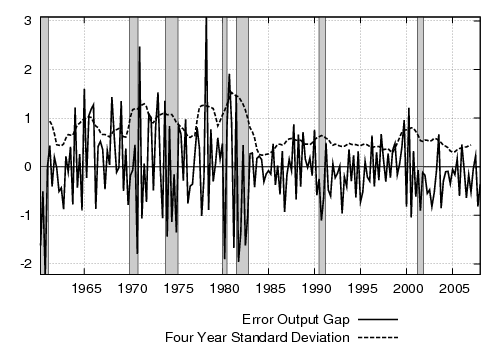
\includegraphics[scale=0.17]{results/results_re/output_err.png} &
  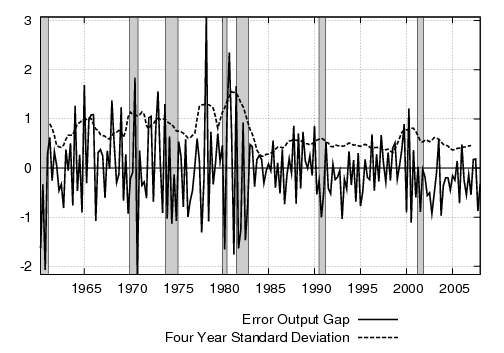
\includegraphics[scale=0.17]{results/results_reallinit/output_err.png} \\ 
  Correlation = 1.0 & Correlation = 0.98 \\
  RMSE = 0.7757 & RMSE = 0.7905 \\ \\
  \textbf{Case 3} & \textbf{Case 4}  \\
  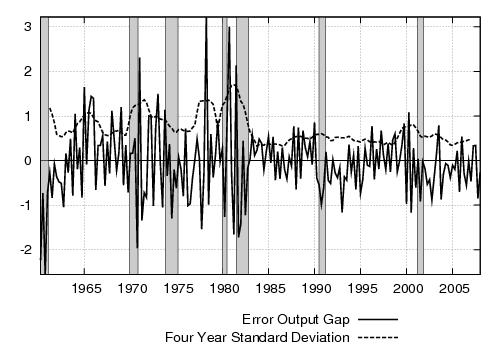
\includegraphics[scale=0.17]{results/results_reinit/output_err.png} &
  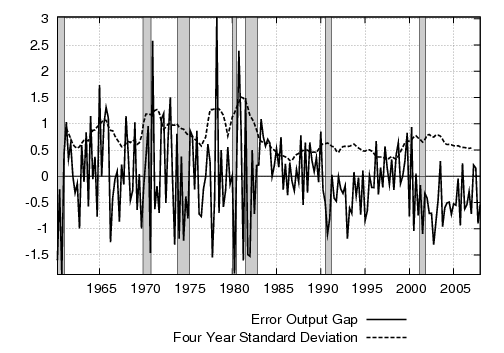
\includegraphics[scale=0.17]{results/results_wlsinit/output_err.png} \\
  Correlation = 0.97 & Correlation = 0.92 \\
  RMSE = 0.8012 & RMSE = 0.7792 \\
  \end{tabular}
  \end{scriptsize}
  \end{center}
  \end{column}

  \begin{column}{1.8in}
  \bi
  \item<+-> RMSE: RE is best fitting model.
  \item<+-> Forecast errors highly correlated with RE.
  \item<+-> All models make larger errors prior to early 1980s.
  \ei
  \end{column}
  \end{columns}
}


\frame {
  \ft{Forecast Errors: Inflation}
  \begin{columns}
  \begin{column}{3in}

  \begin{center}
  \begin{scriptsize}
  \begin{tabular}{cc}
  \textbf{Case 1} & \textbf{Case 2} \\
  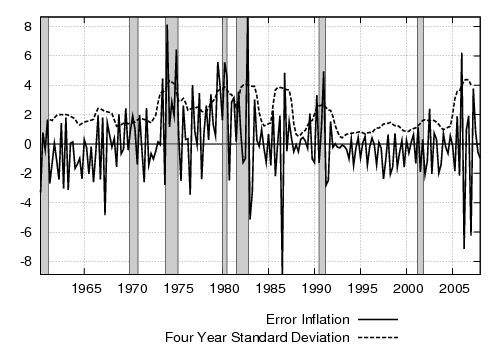
\includegraphics[scale=0.17]{results/results_re/inflation_err.png} &
  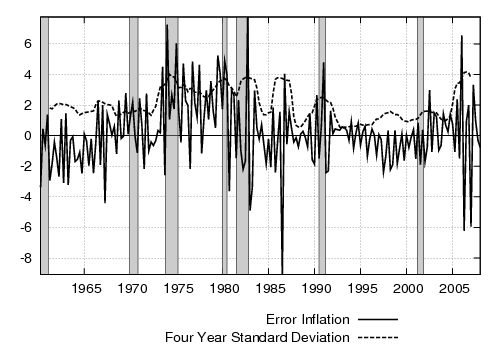
\includegraphics[scale=0.17]{results/results_reallinit/inflation_err.png} \\ 
  Correlation = 1.0 & Correlation = 0.93 \\
  RMSE = 2.3474 & RMSE = 2.2863 \\ \\
  \textbf{Case 3} & \textbf{Case 4} \\
  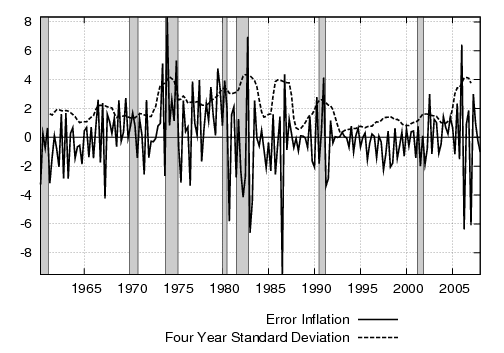
\includegraphics[scale=0.17]{results/results_reinit/inflation_err.png} &
  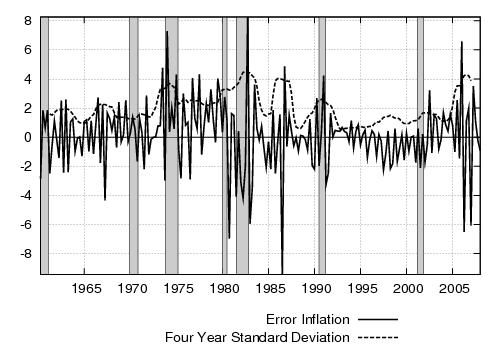
\includegraphics[scale=0.17]{results/results_wlsinit/inflation_err.png} \\
  Correlation = 0.9 & Correlation = 0.89 \\
  RMSE = 2.2978 & RMSE = 2.3092 \\
  \end{tabular}
  \end{scriptsize}
  \end{center}

  \end{column}

  \begin{column}{1.8in}
  \bi
  \item<+-> RMSE: All models provide similar fit to data.
  \item<+-> All models made similar errors
  \item<+-> Largest errors during recessions in 1970s, early 1980s
  \ei
  \end{column}
  \end{columns}
}

\subsection{Impulse Response Functions}
\frame
{
  \ft{Impulse Response Functions}
  \bi
  \item<+-> \textbf{Impulse response function (IRF):} graph of the impact a shock has on a macroeconomic variable.
  \item<+-> Example: positive demand shock 
    \bi
    \item<+-> Causes a temporary positive impact on output and inflation. 
    \item<+-> An IRF shows how large the impact is on each of these variables.
    \item<+-> IRF also shows how long the impacts last.
    \ei
  \item<+-> Learning can impact IRFs as shocks impact agents perceptions of the structure of economy.
    \bi
    \item<+-> Orphanides and Williams (2005) found prolonged inflation IRFs.
    \ei
  \ei    
}

\frame {
  \ft{IRF: Natural Rate Shock on Output}
  \begin{columns}
  \begin{column}{3in}
  \begin{center}
  \begin{tabular}{cc}
  \textbf{Case 1} & \textbf{Case 2}  \\
  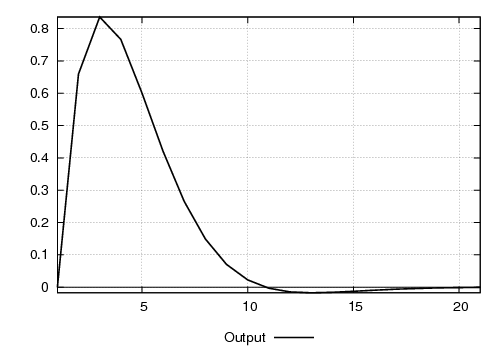
\includegraphics[scale=0.2]{results/results_re/Output_natshock_irf.png} &
  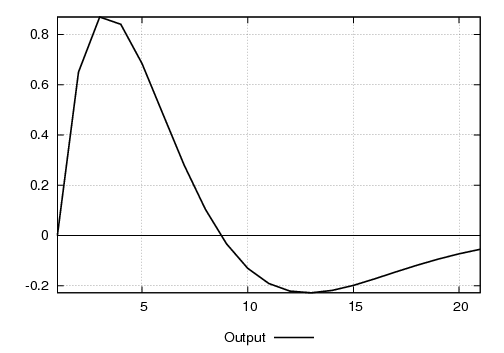
\includegraphics[scale=0.2]{results/results_reallinit/Output_natshock_irf.png} \\ \\
  \textbf{Case 3} & \textbf{Case 4} \\
  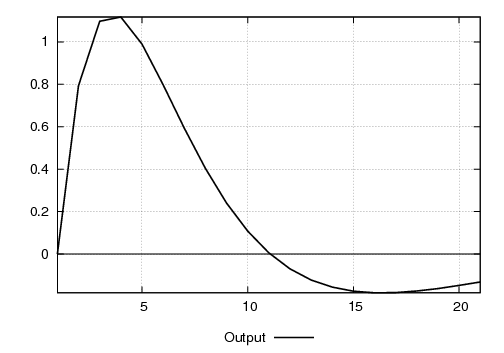
\includegraphics[scale=0.2]{results/results_reinit/Output_natshock_irf.png} &
  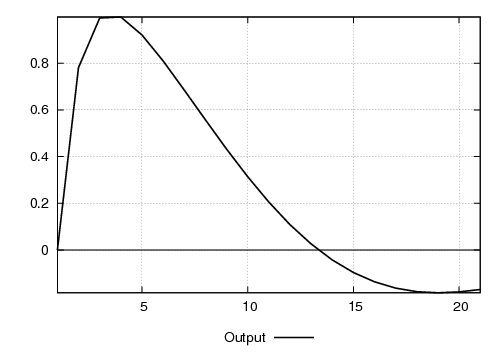
\includegraphics[scale=0.2]{results/results_wlsinit/Output_natshock_irf.png} \\
  \end{tabular}
  \end{center}
  \end{column}

  \begin{column}{1.8in}
  \bi
  \item<+-> Learning leads to prolonged effects on output.
  \item<+-> Learning without knowledge of shocks leads to oscillatory effects.
  \ei
  \end{column}
  \end{columns}
}

\frame 
{
  \ft{IRF: Natural Rate Shock on Inflation}
  \begin{columns}
  \begin{column}{3in}
  \begin{center}
  \begin{tabular}{cc}
  \textbf{Case 1} & \textbf{Case 2}  \\
  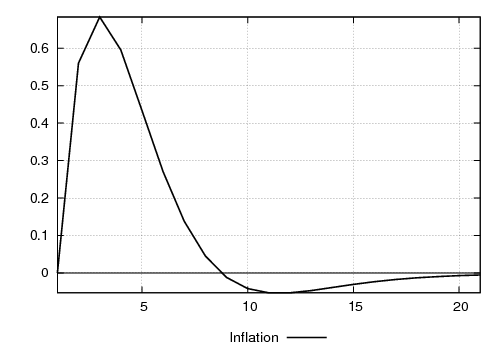
\includegraphics[scale=0.2]{results/results_re/Inflation_natshock_irf.png} &
  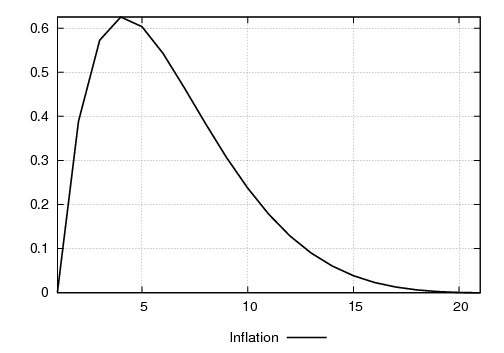
\includegraphics[scale=0.2]{results/results_reallinit/Inflation_natshock_irf.png} \\ \\
  \textbf{Case 3} & \textbf{Case 4} \\
  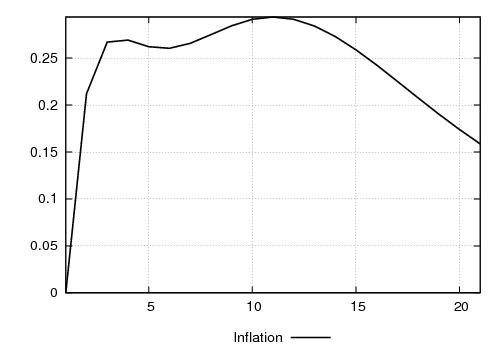
\includegraphics[scale=0.2]{results/results_reinit/Inflation_natshock_irf.png} &
  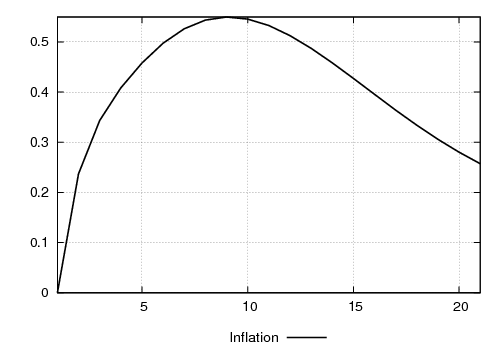
\includegraphics[scale=0.2]{results/results_wlsinit/Inflation_natshock_irf.png} \\
  \end{tabular}
  \end{center}

  \end{column}

  \begin{column}{1.8in}
  \bi
  \item<+-> Learning can lead to very prolonged effects on inflation.
  \item<+-> Learning without knowledge of shocks leads to long lasting oscillatory effects.
  \ei
  \end{column}
  \end{columns}
}

\frame
{
  \ft{Time-varying Impulse Responses}
  \bi
  \item<+-> Under rational expectations - agents always know structure of the economy, therefore impulse responses are always the same.
  \item<+-> Under learning - impulse responses depend on the state of expectations.
  \item<+-> Previous slides - showed the impulse responses for the last sample period (2008:Q1).
  \item<+-> Next slides - 3-D impulse response functions, showing what the impulse response function looked like at each period in the sample. 
  \ei
}

\frame {
  \ft{Case 2: Natural Rate Shock on Output}
  \hspace*{-0.35in}
  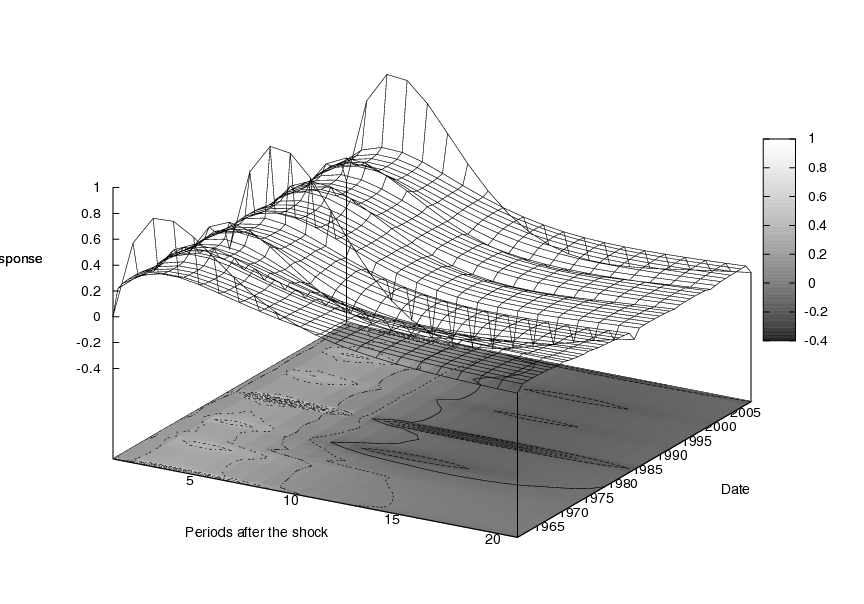
\includegraphics[scale=0.4]{results/results_reallinit/Output_natshock_irf3d.png} 
}

\frame {
  \ft{Case 3: Natural Rate Shock on Output}
  \hspace*{-0.35in}
  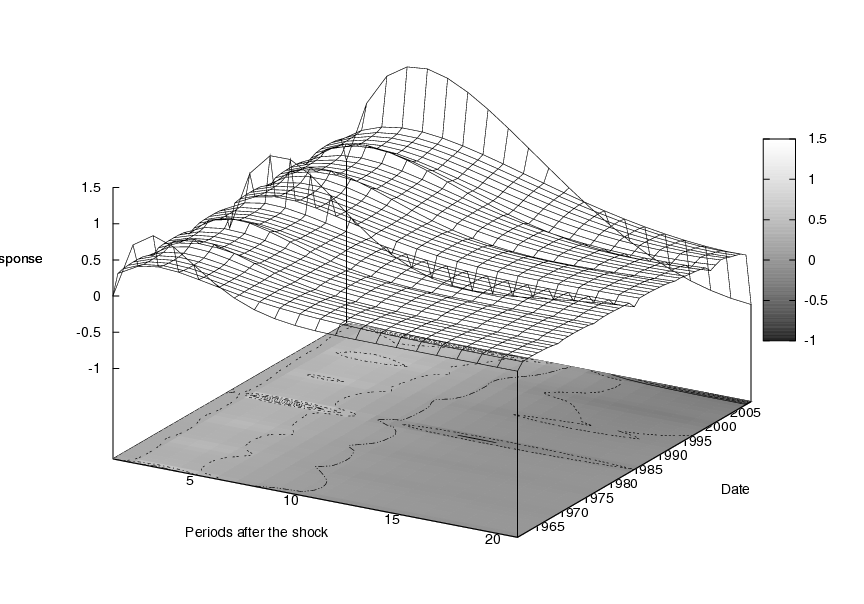
\includegraphics[scale=0.4]{results/results_reinit/Output_natshock_irf3d.png} 
}

\frame {
  \ft{Case 4: Natural Rate Shock on Output}
  \hspace*{-0.35in}
  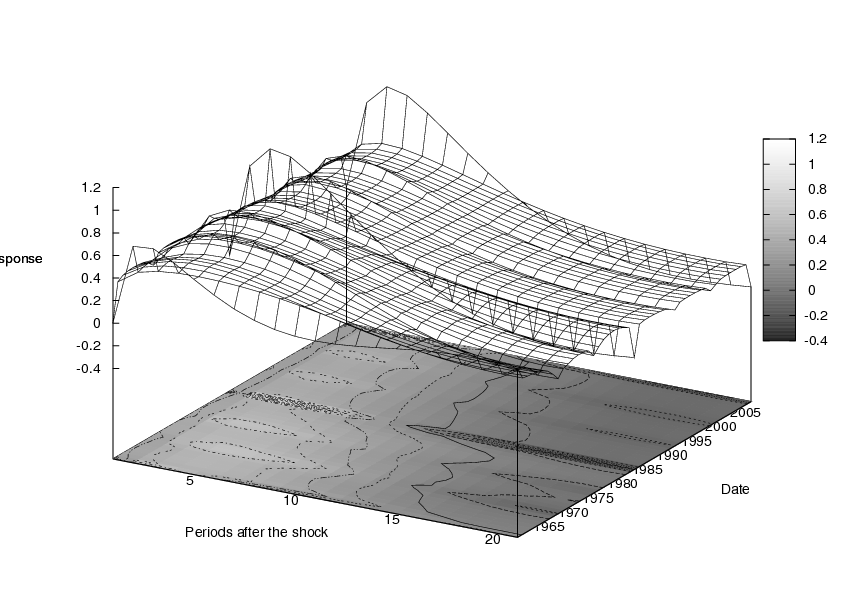
\includegraphics[scale=0.4]{results/results_wlsinit/Output_natshock_irf3d.png} 
}

\frame {
  \ft{Case 2: Natural Rate Shock on Inflation}
  \hspace*{-0.35in}
  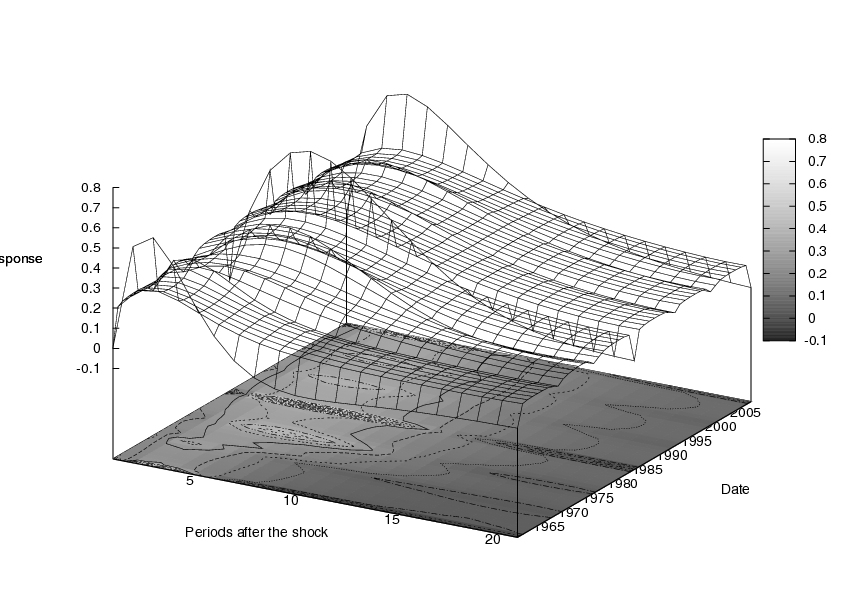
\includegraphics[scale=0.4]{results/results_reallinit/Inflation_natshock_irf3d.png} 
}
\frame {
  \ft{Case 3: Natural Rate Shock on Inflation}
  \hspace*{-0.35in}
  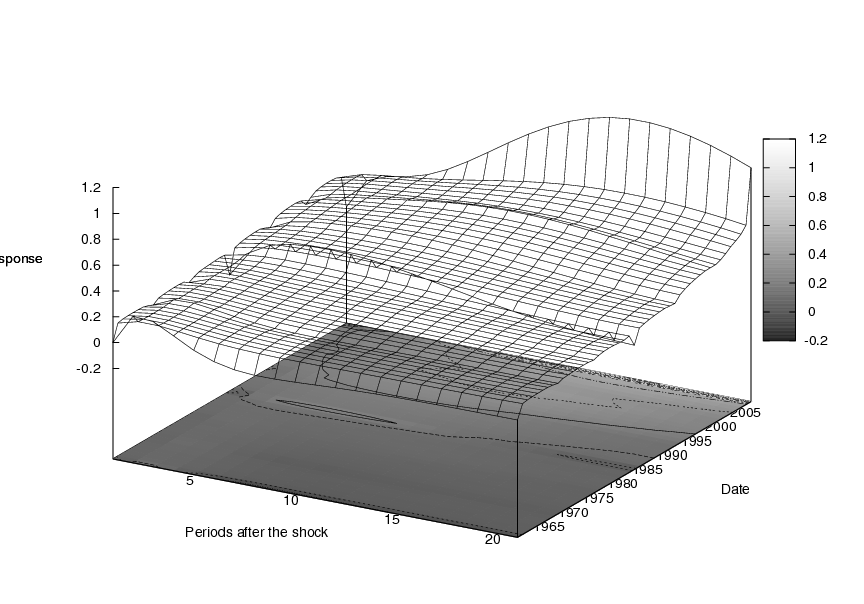
\includegraphics[scale=0.4]{results/results_reinit/Inflation_natshock_irf3d.png} 
}

\frame {
  \ft{Case 4: Natural Rate Shock on Inflation}
  \hspace*{-0.35in}
  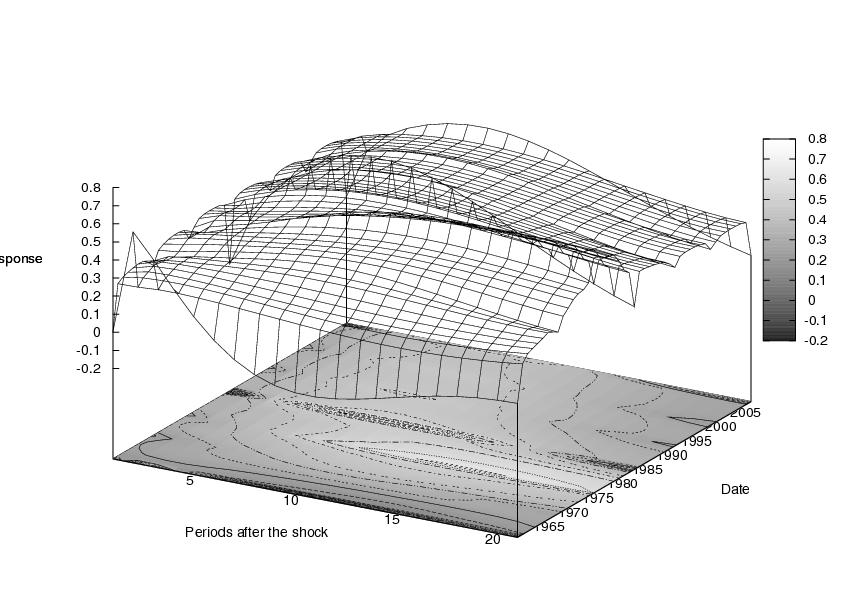
\includegraphics[scale=0.4]{results/results_wlsinit/Inflation_natshock_irf3d.png} 
}

\frame
{
  \ft{Time Varying Impulse Responses}
  \bi
  \item<+-> Impulse responses are more prolonged in cases 3 and 4 (when agents do not observe structural shocks).
  \item<+-> Impulse responses are largest during recessions of 1970s, early 1980s, and especially 2008:Q1.
  \ei
}

\section{}
\subsection{Conclusions}
\frame
{
  \ft{Conclusions}
  \bi
  \item<+-> Learning gain is statistically significant.
  \item<+-> Otherwise minimal evidence of learning over RE.
  \item<+-> Incorporating learning leads to parameter estimates that imply less sensitivity to expectations.
  \item<+-> Largest errors for every specification still occur during 1970s and early 1980s.
  \item<+-> Learning + Limited information sets leads to prolonged and oscillatory impulse responses. 
  \item<+-> 3D Impulse Responses show the United States was more sensitive to shocks following recessions in 1970s, early 1980s, and now.
  \ei
}

\end{document}

